\section{A Multimodal Target-Source Classifier With Attention Branches
to Understand Ambiguous Instructions for Fetching Daily
Objects}\label{header-n258}

\emph{IEEE ROBOTICS AND AUTOMATION LETTERS, VOL. 5, NO. 2, APRIL 2020}
{[}29{]}

\subsection{Introduction}\label{header-n260}

In the last few years, the domestic service robots (DSRs) have become
more popular: they have a lot of different and useful functions and they
can help people with disabilities. Despite this, one of the main
limitations of DSRs is their inability to naturally interact through
natural language. This ability may be appreciated by non-expert users. A
particular task like various expressions relating to an object for
fetching tasks. This work focuses on \emph{multimodal language
understanding for fetching instructions} (MLU-FI). This task consists of
predicting a target instructed in natural language, such as ``\emph{Bring
me the yellow box from the wooden cabinet.}". The purpose is to
understand how to extract instructions for robots from natural-language
expressions. Natural language induces ambiguity because of the
many-to-many mapping between the linguistic and physical world which
makes it difficult to accurately infer the user's intention. In this
work, the authors propose the multimodal target-source classifier model
with the attention branch (MTCM-AB) which is an extension of the MTCM
(proposed in {[}5{]}), with the addition of the attention branch network
(ABN) explained in {[}6{]}. The MTCM module predicts the region-wise
likelihood of target and source candidates in the scene. Unlike other
methods, MTCM can handle region-wise classification based on linguistic
and visual features. The ABN is an image classifier, inspired by class
activation mapping (CAM) structures, that generates attention maps. This
line of research focuses on the production of image masks that, overlaid
onto an image, highlight the most salient portions with respect to some
given query or task. An attention map is an image with highlighted the
salient regions of a given label. Multiple visual attention networks
were also proposed in recent years for solving visual question
answering. However, most of these approaches use only a single modality
for attention: visual attention. By contrast, recent studies in
multimodal language understanding have shown that both linguistic and
visual attention is beneficial for the given task.

\subsection{Problem definition}\label{header-n262}

The aim is to predict a target referred by an initial instruction among
a set of candidate targets in a visual scene. Instructions are not
constrained which is more natural but increases the complexity of the
comprehension task because users may use referring expressions to
characterize a target. Examples of possible instruction can be:
``\emph{Take the Kleenex box and put it in the bottom right box}" or
``\emph{Go to the kitchen and take the tea bottle on the upper shelf}".
To address the MLU-FI are considered:

\begin{itemize}
\item
  \textbf{Input:} a fetching instruction as a sentence in addition to an
  image of the scene. 
\item
  \textbf{Output:} the most likely target-source pair. The terms target
  and source are defined as follows.

  \begin{itemize}
  \item
    \textbf{Target:} a daily object (e.g. bottle or snacks) that a user
    intends the robot to fetch.
  \item
    \textbf{Source:} the origin of the target (e.g. desk or cabinet).
  \end{itemize}
\end{itemize}

The evaluation metric is the prediction accuracy over the top-1 target
prediction. Ultimately this study does not focus on object detection.
The authors suppose that the bounding boxes of the target and source are
given in advance. The MTCM-AB is not specifically designed for a given
scene or context. It is validated on two types of datasets, in real and
simulated environments described below.

\begin{itemize}
\item
  \textbf{Home Environment:} In this configuration, the experiments use
  a simulation-based dataset from the Partner Robot Challenge Virtual
  Space (WRS-PV). WRS-PV depicts home environments as represented in the
  figure below. The three-dimensional environments (Unity-based) are
  augmented to make them more realistic. In this environment, a targeted
  DSR, that is HSR (Human Support Robot), can freely navigate and
  manipulate objects. In this context, the MTCM-AB predicts the most
  likely target among several candidates.
\item
  \textbf{Pick-and-Place Scene:} the PFN-PIC {[}7{]} dataset is designed
  for pick-and-place tasks from an armed robot with a top-view camera.
  The scene consists of four boxes, in which several candidate targets
  (up to 40) are randomly placed.
\end{itemize}

\begin{figure}[h!]
\centering
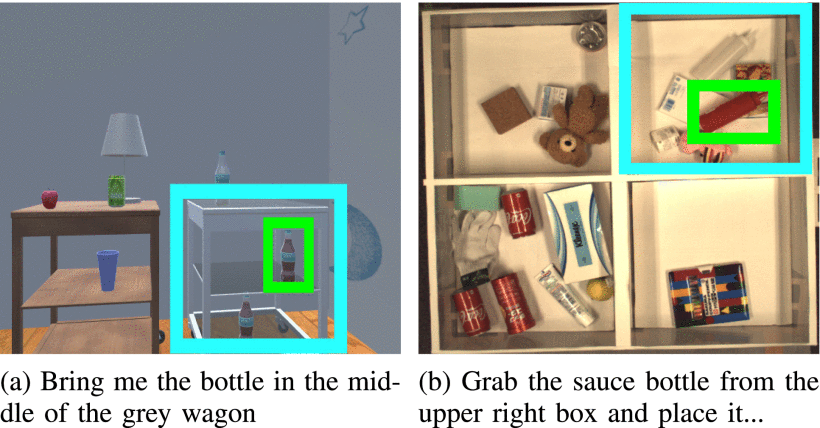
\includegraphics[width=0.8\linewidth]{images/WRS-PVexample.png}
\caption{Samples of the WRS-PV (left) and PFN-PIC datasets (right) where the source and target are given.}
\end{figure}

\subsection{Proposed method}\label{header-n281}

The proposed method consists of target prediction with respect to
instruction in natural language. The authors extend the MTCM {[}5{]}
with an attention branch network (ABN, {[}6{]}) that are used to improve
the prediction from the linguistic and visual inputs. In ABN, the class
attention map (CAM) network is extended to produce an attention mask for
improving image classification. The ABN is decomposed into parallel
branches to avoid deteriorating the classifier accuracy (both of them
are classifiers):

\begin{itemize}
\item
  an attention branch that produces attention maps and
\item
  a prediction branch that predicts the likelihood of some label.
\end{itemize}

The MTCM-AB module produced in this work, similarly to the MTCM,
predicts the target and source from the full sentence. This module is
composed of a set of sub-modules: the Target Attention Branch (TAB), the
neighboring Context Attention Branch (nCAB), and the Linguistic
Attention Branch (LAB). The MTCM-AD architecture is explained in detail
in the following line and the figure below is a visual representation of
it. The MTCM module works as follow:

\begin{itemize}
\item
  \textbf{Input:} for each target candidate $i \in \{1, . . ., N\}$
  and source $i^{'} \in \{1, . . ., M\}$, the input is

  $ {\mathbf x}(i)=\lbrace {\mathbf x}_{l}(i), {\mathbf x}_{t} (i), {\mathbf x}_{c} (i), {\mathbf x}_{r} (i) \rbrace, $

  where ${\mathbf x}_l(i)$, ${\mathbf x}_t(i)$, ${\mathbf x}_c(i)$ and
  ${\mathbf x}_r(i)$ denote linguistic, target, context and relation
  features. The authors purposefully omit index in the following, that
  is, ${\mathbf x}(i)$ is then written as ${\mathbf x}$. More in detail, the
  input variables define:

  \begin{itemize}
  \item
    ${\mathbf x}_t(i)$: it is defined as the cropped image of the target
  \item
    ${\mathbf x}_c(i)$: it is a cropped image that characterizes a target
    and its neighborhood (context)
  \item
    ${\mathbf x}_c(l)$: it consists of sub-word vector embedding
  \item
    ${\mathbf x}_r(i)$: it is a vector characterizing the position of the
    target candidate in the environment.
  \end{itemize}
\item
  \textbf{Linguistic Attention Branch (LAB):} its purpose is to
  emphasize the most salient part of the linguistic features for
  instruction comprehension. The LAB module is composed by a
  implementation of the BERT method for the sub-word embedding (extract
  the words internal structure). Subsequently, the multi-layer Bi-LSTM
  network is used to obtain a latent space representation of the
  extracted linguistic features. The last hidden states of each layer
  are concatenated to form \emph{linguistic feature maps}
  f\textsubscript{l}, from which a linguistic attention mask is
  extracted. Feature maps f\textsubscript{l} are processed through
  one-dimensional convolutional layers followed by a single fully
  connected layer (FC) The \emph{linguistic attention map}
  a\textsubscript{l} is obtained from the second convolutional layer
  that is convoluted with an additional layer and normalized by a
  sigmoid activation function. The output visual feature maps are then
  obtained using a masking process given by

  $ {\mathbf o}_{l}= {\mathbf a}_l \odot {\mathbf f}_{l} $

  where $\odot$ denotes the Hadamard product (takes two matrices of
  the same dimensions and produces another matrix of the same dimension
  as the operands where each element $i, j$ is the product of elements
  $i, j$ of the original two matrices).
\item
  \textbf{Target Attention Branch (TAB):} it produces an attention map
  for the candidate target images. The input ${\mathbf{x}_t}$ is
  transformed into a space feature ${\mathbf{f}_t}$ through a CNN, which
  is processed into FC layers. Even in this case, a visual attention map
  is extracted from the second FC layer that is processed in a parallel
  branch composed of a FC layer and a sigmoid activation function.
  Output latent space feature o\textsubscript{t} is then obtained by

  $ {\mathbf o}_{t}= {\mathbf a}_t \odot {\mathbf f}_{t}.$
\item
  \textbf{Neighboring Context Attention Branch: (nCAB):} it is one of
  the main novelties of the MTCM-AB. nCAB module adds an attention
  branch mechanism to focus on the relevant part of the image in the
  surroundings of a given target, in order to define context features.
  An extended cropped image (${\mathbf x}_c$) is extracted from around the
  target. This input is encoded into feature maps ${\mathbf{f}_c}$ from a
  CNN feature extractor. The convolutional layers are followed by a
  global average pooling (GAP). In parallel, context attention map
  a\textsubscript{c} is created from an additional convolution and
  sigmoid normalization of the third convolutional layer. The output
  context feature maps are given by

  $ {\mathbf o}_{c}= {\mathbf a}_{c} \odot {\mathbf f}_{c}.$
\item
  \textbf{Perception Branch:} it is composed by a visual multi-layer
  perceptron (MLP), which encodes the concatenation of ${\mathbf{o}_t}$,
  ${\mathbf{o}_v}$ and ${\mathbf{x}_r}$. In parallel, a linguistic MLP
  encodes linguistic features ${\mathbf{o}_l}$. The source is predicted as
  ${\mathbf{J}_{src}}$ from a third MLP that combines the two previous MLP
  outputs.
\item
  \textbf{Loss Functions:} the MTCM-AB is trained by minimizing several
  embedding loss functions related to the different branches. In
  particular, it minimizes the global loss function
  $J_{total} = \lambda_cJ_c + \lambda_tJ_t + \lambda_lJ_l + \lambda_pJ_p + \lambda_{src}J_{src}$,
  where J\textsubscript{i} is the loss function for the branch i and
  $\lambda_i$ are loss weights that are defined in the experimental
  section.
\end{itemize}

\begin{figure}[h!]
\centering
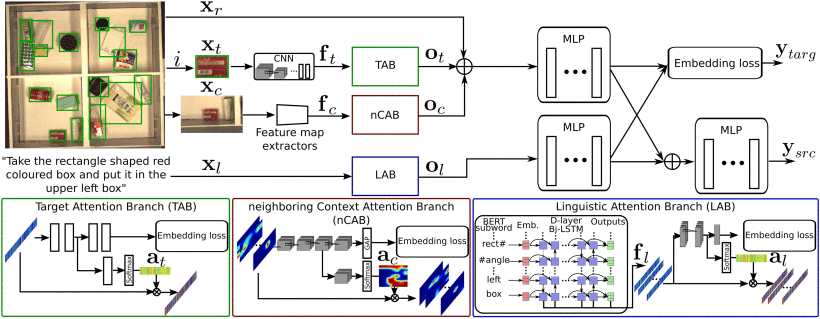
\includegraphics[width=0.8\linewidth]{images/MTMC-AB.png}
\caption{MTCM-AB architecture}
\end{figure}

\subsection{Experiments}\label{header-n318}

The proposed method is evaluated over the PFN-PIC and WRS-PV datasets.
The first contains 89,891 sentences in the training set and 898
sentences in the validation set to instruct 25,861 targets in the
training set and 532 targets in the validation one. The latter, instead,
has 308 images from which 2015 instructions in the training set and 74
instructions in the validation set. The experimental setup is summarized
in the following figure. This configuration is used to train the model
with the PFN-PIC dataset, while for the WRSPV dataset the learning rate
was decreased to $5 \times 10^{-5}$ and a batch size of 64.

\begin{figure}[h!]
\centering
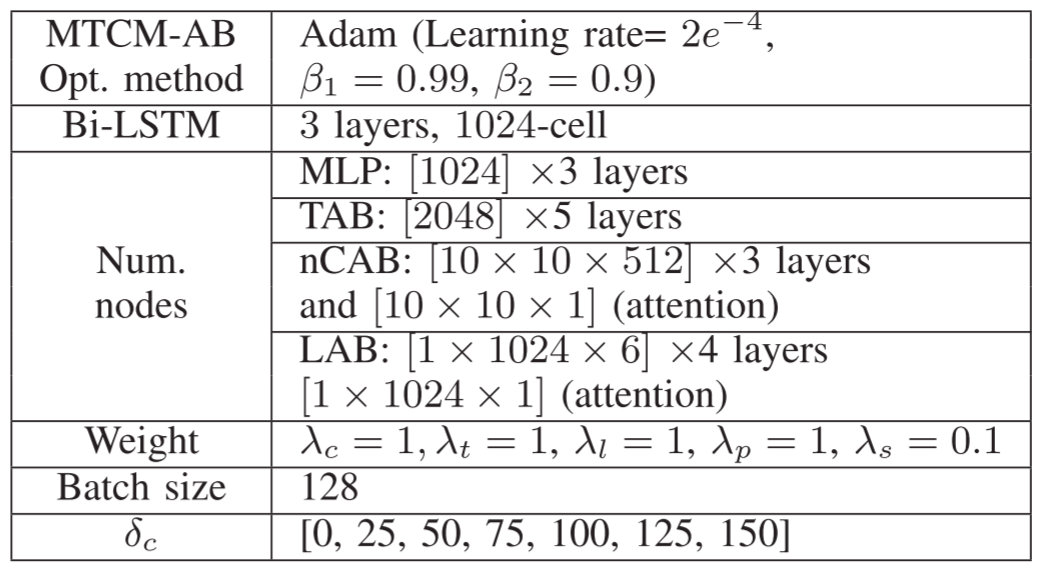
\includegraphics[width=0.85\linewidth]{images/MTCMsettings.png}
\caption{MTCM-AB settings parameters}
\end{figure}

The input images were downscaled to $299 \times 299$ before being processed.
The parameter $\delta_c$ represents the variation in size of the
context input ${\mathbf x}_c$. It corresponds to the size of the cropped
image target to which is added $\delta_c$ in width and height. The
MTCM-AB had 27.5 M parameters.

\newpage
\subsection{Results}\label{header-n322}

\subsubsection{Quantitative results}\label{header-n323}

The \emph{quantitative results} correspond to the accuracy obtained for
the most likely target predicted, given an instruction. This metrics is
also called \emph{top-1 accuracy}. The authors report the performance
variation with varying sizes of ${\mathbf x}_c$ by setting $\delta_c$
with a 0 to 150-pixel wise extension, to find the best value of
$\delta_c$. These results are reported in the following figure.

\begin{figure}[h!]
\centering
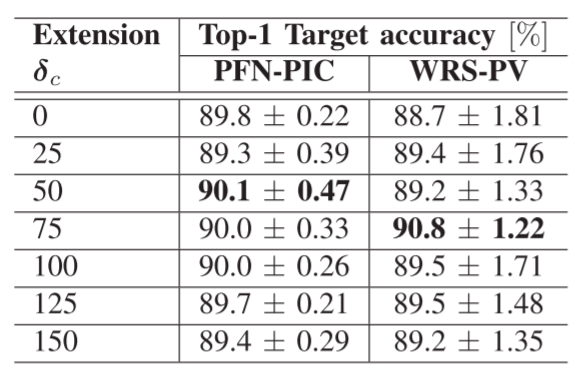
\includegraphics[width=0.65\linewidth]{images/MTCMresultssize.png}
\caption{MTCM-AB accuracy with respect to $\delta_c$}
\end{figure}

From $\delta_c$ analysis, the authors found its best value for the two
datasets, which is, respectively, 50 and 75 pixels for the PFN-PIC and
WRS-PV datasets. In addition, this analysis shows that the PFN-PIC
dataset is highly cluttered with relatively small objects, because
setting $\delta_c = [125, 150]$ causes lower accuracy than the
configuration with $\delta_c = 0$. The MTCM-AB method proposed in this
work is compared with respect to other state-of-the-art models and human
performance, which is considered as an upper bound. These confront
models are the MTCM {[}1{]} and its baseline method explained in {[}7{]}
by Hatori et al. The results, in terms of top-1 accuracy, are reported
in the following figure.

\begin{figure}[h!]
\centering
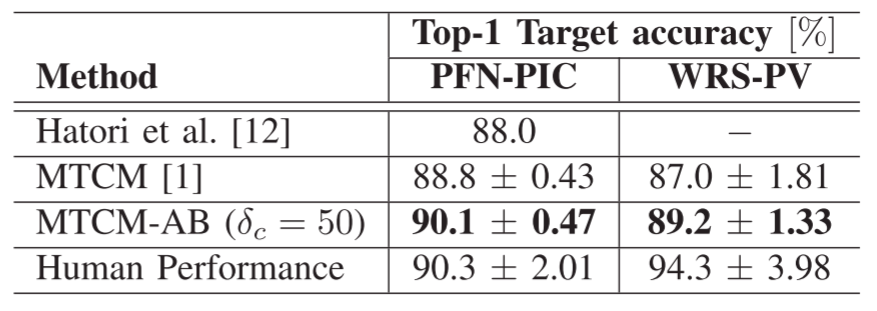
\includegraphics[width=0.75\linewidth]{images/MTCMqualres.png}
\caption{Top-1 Accuracy on PFN-PIC and WRS-PV datasets}
\end{figure}

On PFN-PIC, the MTCM-AB outperformed the MTCM and baseline method by
1.3\% and 2.1\% respectively. The results of WRS-PV corroborated the
trend observed on the PFN-PIC dataset. To characterize the contribution
of each attention branch, the authors also report the results of an
ablation study for the PFN-PIC dataset. These results, showed in the
following figure, show that both linguistic and visual attention
branches improved the prediction accuracy compared to the MTCM.

\begin{figure}[h!]
\centering
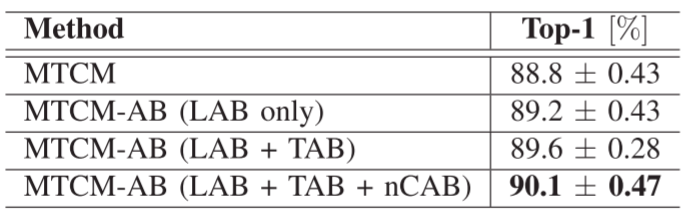
\includegraphics[width=0.75\linewidth]{images/MTCMablanation.png}
\caption{Ablanation study of the MTCM-AB for PFN-PIC dataset}
\end{figure}

\subsubsection{Qualitative Results}\label{header-n330}

In the following figure, the \emph{qualitative results} are reported for
the PFN-PIC dataset. In the first row, the prediction is given in blue
while the ground truth is in green. The attended region of each context
feature ${\mathbf x}_c$ is given in the second row. The two first columns
refer to correct predictions. The third column refers to an erroneous
prediction (wrongly attended target), while the last column refers to an
erroneous prediction due to incorrect ground truth (``brown pack" is
instructed but ``can" is given the label). The sentences are:

\begin{itemize}
\item
  ``\emph{Take the blue sandal move it to lower left box}"
\item
  ``\emph{Take the green item next to the pair of white gloves and move
  it to top left box}"
\item
  ``\emph{Move the grey colored bottle at top left to box below}"
\item
  ``\emph{Pick the brown pack and put it in lower left box}"
\end{itemize}
\newpage
\begin{figure}[h!]
\centering
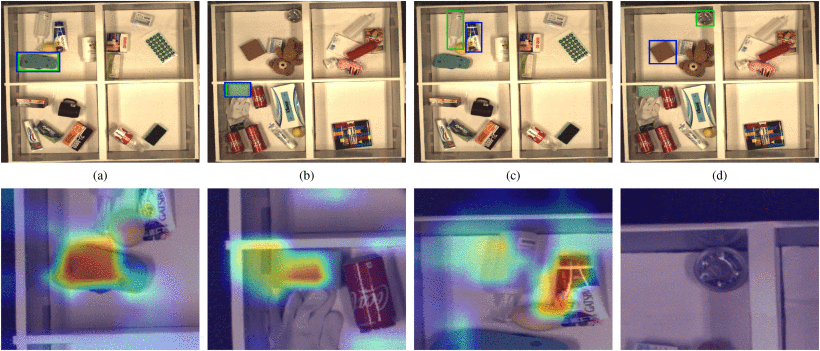
\includegraphics[width=0.8\linewidth]{images/MTMCqualres1.png}
\caption{Qualitative results for PFN-PIC dataset}
\end{figure}

Qualitative results on the WRS-PV dataset are analyzed in the same way.
The three first samples illustrate correct predictions with consistent
attended regions. The last sample, with the instruction ``Take an apple
on the same shelf that a coffee cup is placed is erroneous and our
model predicts the cup instead of the apple.

\begin{figure}[h!]
\centering
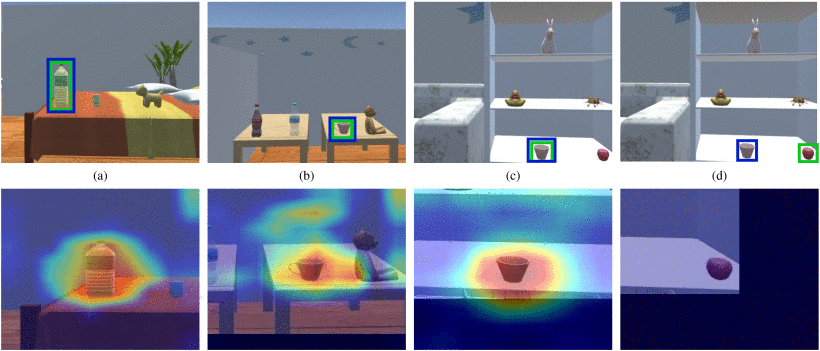
\includegraphics[width=0.8\linewidth]{images/MTMCqualres2.png}
\caption{Qualitative results for WRS-PV dataset}
\end{figure}

\subsubsection{Error Analysis}\label{header-n344}

Analysing the MTCM-AB results, different failure cases can be observed:

\begin{itemize}
\item
  \textbf{ES (erroneous sentence):} the ground truth does not correspond
  to the target specified in the instruction
\item
  \textbf{NE (negation):} the ground truth is specified from a negation
  sentence which is thought to be difficult to solve in NLP community
\item
  \textbf{REL (relation to landmark):} the ground truth is defined with
  respect to landmark objects and the predicted target position is
  incorrect with respect to this landmark
\item
  \textbf{RES (relation to source):} the ground truth target is defined
  with respect to a source and the predicted target position is
  incorrect with respect to this source
\item
  \textbf{SE (source error):} the instruction specifies a given source
  and the predicted target position is in a different source
\end{itemize}